\documentclass[12pt, letterpaper]{article}
\usepackage{graphicx}
\setlength{\parindent}{0pt}

\begin{document}
  % Title page
  \begin{titlepage} 
    \begin{center}
      \Huge{\textbf{Lab 1}}\\
      \Huge{Motion diagrams}
      \vfill
      \large{\textbf{Rectangle Repulsed Researchers}}\\
      \large{Julian Barossi, Liam Gilligan, Stephanie L'Heureux}\\
      \vspace*{0.5cm}
      \normalsize
      \today
    \end{center}
  \end{titlepage}

  % Section title 
  \begin{center}
    \rule{\textwidth}{0.5pt}
    \normalsize{\textbf{Part 3:} Matching Position vs. Time and Velocity vs. Time Graphs}\\
    \vspace{0.5cm}
  \end{center}

  % Begin subsection
  \begin{center}
    \Large\textbf{{Graph 1}}\\
  \end{center}


  \large{Graph discription}\\
  Graph one depicts a the position vs time graph 
  Graph 1 shows a graph of a collision. The object's distance from the sensor 
  is increasing. The slope of the position is velocity so we can also say 
  that the velocity is positive and constant. Then at $t\approx2.4s$ its position
  begins decreasing at a constant, negative velocity.\\ 
  \begin{equation} 
    \indent{} \frac{d}{dx}[s(t)] =  v_{x_1} = 0.35m/s
    \indent{}V_{x_2}= -0.35m/s
  \end{equation}\\
  \large{Setup}\\
  Our setup consisted as a flat track with a magnetic bumper $60cm$ from the
  the \emph{PASCO Universal 850 interface and Motion Sensor II}. We pushed and released the cart towards the bumper. 
  We consider friction and drag negligible.\\

  \large{Graph 2:}\\
  \large{Graph discription:}\\
  \noindent{Graph 2 depicts an object speeding up at a constant rate. We know this because the
  object's position is increasing and the velocity is positive and increasing.}\\
  \large{Setup:}\\
  Our setup consisted of a track at an downward incline. We released the cart from the 
  top of the track and let it slide to the bottom. We consider friction and drag negligible.\\

  \large{Graph 3:}\\
  \large{Graph discription:}\\
  \noindent{Graph 3 depicts an object in freefall that hits the ground and stays there. We know this because the
  object's position starts from an increased height}\\
  \large{Setup:}\\
  Our setup consisted of a the sensor positioned updward. We dropped a large beach ball.\\

  \large{Graph 4:}\\
  \large{Graph discription:}\\
  \noindent{Graph 4 depicts an object moving down an incline. It comes in contact with somethinhg at the bottom and changes direction. As it changes direction it slows down. Then at $t=2.6s$ its velocity becomes negaiive but the acceleration staus positive where it is slowing down}\\
  \large{Setup:}\\
  Our setup consisted of a the sensor positioned at the biotton of an incline plane. We released the cart from the top 


  \large{Graph 5:}\\
  \large{Graph discription:}\\
  \noindent{Graph 5 depicts an object that starts from rest then is that ts pushed then slows to a stop. 
  We know this because the graph depicts the initial velocity as 0m/s, then the velocity rapidluy increases and the acceleration is posiyive. It the acceleratyion goes to zero and he velocity is constant}\\
  \large{Setup:}\\
  Our setup consisted a flat plane and w pushed the cart away from the sensor

  \large{Graph 6:}\\
  \large{Graph discription:}\\
  \noindent{Graph 6 depicts an object which is pushed and released up a hill. Eventually gravity slows it down and it 
  returns down the hill}\\
  \large{Setup:}\\
  Our setup consisted of a incline plane. We gave the cart a push and let it go up the hill then return down

  \large{Graph 6:}\\
  \large{Graph discription:}\\
  Graph 6 depicts an object moving up and swown on a spring.\\
  \large{Setup:}\\
  Our setup consisted of an downward incline. The bumper was positioned $60cm$ away from the sensor.  








  % \centerline{\textbf{Graph 1}}\\
  % % Any kind of straight lines, calculate a slope. D
  % \textbf{Graph 2}\\
  % \textbf{Graph 3}\\
  % \textbf{Graph 4}\\
  % \textbf{Graph 5}\\
  % \textbf{Graph 6}\\
  % \textbf{Graph 7}\\

  % \centerline{}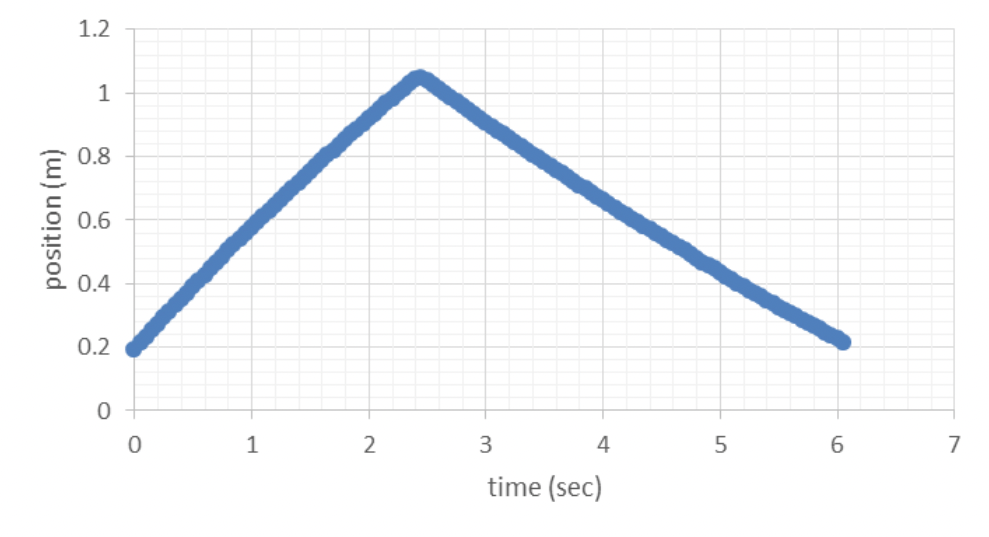
\includegraphics{graph_1.png}}

\end{document}
